\documentclass{report}
\usepackage{graphicx}
\graphicspath{ {imagenes/} }
\usepackage[utf8]{inputenc}
\makeatletter
\usepackage{color}
\definecolor{lightgray}{rgb}{0.95, 0.95, 0.95}
\definecolor{darkgray}{rgb}{0.4, 0.4, 0.4}
%\definecolor{purple}{rgb}{0.65, 0.12, 0.82}
\definecolor{editorGray}{rgb}{0.95, 0.95, 0.95}
\definecolor{editorOcher}{rgb}{1, 0.5, 0} % #FF7F00 -> rgb(239, 169, 0)
\definecolor{editorGreen}{rgb}{0, 0.5, 0} % #007C00 -> rgb(0, 124, 0)
\definecolor{orange}{rgb}{1,0.45,0.13}		
\definecolor{olive}{rgb}{0.17,0.59,0.20}
\definecolor{brown}{rgb}{0.69,0.31,0.31}
\definecolor{purple}{rgb}{0.38,0.18,0.81}
\definecolor{lightblue}{rgb}{0.1,0.57,0.7}
\definecolor{lightred}{rgb}{1,0.4,0.5}
\usepackage{upquote}
\usepackage{listings}
% CSS
\lstdefinelanguage{CSS}{
  keywords={color,background-image:,margin,padding,font,weight,display,position,top,left,right,bottom,list,style,border,size,white,space,min,width, transition:, transform:, transition-property, transition-duration, transition-timing-function},	
  sensitive=true,
  morecomment=[l]{//},
  morecomment=[s]{/*}{*/},
  morestring=[b]',
  morestring=[b]",
  alsoletter={:},
  alsodigit={-}
}

% JavaScript
\lstdefinelanguage{JavaScript}{
  morekeywords={typeof, new, true, false, catch, function, return, null, catch, switch, var, if, in, while, do, else, case, break},
  morecomment=[s]{/*}{*/},
  morecomment=[l]//,
  morestring=[b]",
  morestring=[b]'
}

\lstdefinelanguage{HTML5}{
  language=html,
  sensitive=true,	
  alsoletter={<>=-},	
  morecomment=[s]{<!-}{-->},
  tag=[s],
  otherkeywords={
  % General
  >,
  % Standard tags
	<!DOCTYPE,
  </html, <html, <head, <title, </title, <style, </style, <link, </head, <meta, />,
	% body
	</body, <body,
	% Divs
	</div, <div, </div>, 
	% Paragraphs
	</p, <p, </p>,
	% scripts
	</script, <script,
  % More tags...
  <canvas, /canvas>, <svg, <rect, <animateTransform, </rect>, </svg>, <video, <source, <iframe, </iframe>, </video>, <image, </image>, <header, </header, <article, </article
  },
  ndkeywords={
  % General
  =,
  % HTML attributes
  charset=, src=, id=, width=, height=, style=, type=, rel=, href=,
  % SVG attributes
  fill=, attributeName=, begin=, dur=, from=, to=, poster=, controls=, x=, y=, repeatCount=, xlink:href=,
  % properties
  margin:, padding:, background-image:, border:, top:, left:, position:, width:, height:, margin-top:, margin-bottom:, font-size:, line-height:,
	% CSS3 properties
  transform:, -moz-transform:, -webkit-transform:,
  animation:, -webkit-animation:,
  transition:,  transition-duration:, transition-property:, transition-timing-function:,
  }
}

\lstdefinestyle{htmlcssjs} {%
  % General design
%  backgroundcolor=\color{editorGray},
  basicstyle={\footnotesize\ttfamily},   
  frame=b,
  % line-numbers
  xleftmargin={0.75cm},
  numbers=left,
  stepnumber=1,
  firstnumber=1,
  numberfirstline=true,	
  % Code design
  identifierstyle=\color{black},
  keywordstyle=\color{blue}\bfseries,
  ndkeywordstyle=\color{editorGreen}\bfseries,
  stringstyle=\color{editorOcher}\ttfamily,
  commentstyle=\color{brown}\ttfamily,
  % Code
  language=HTML5,
  alsolanguage=JavaScript,
  alsodigit={.:;},	
  tabsize=2,
  showtabs=false,
  showspaces=false,
  showstringspaces=false,
  extendedchars=true,
  breaklines=true,
  % German umlauts
  literate=%
  {Ö}{{\"O}}1
  {Ä}{{\"A}}1
  {Ü}{{\"U}}1
  {ß}{{\ss}}1
  {ü}{{\"u}}1
  {ä}{{\"a}}1
  {ö}{{\"o}}1
}
%
\lstdefinestyle{py} {%
language=python,
literate=%
*{0}{{{\color{lightred}0}}}1
{1}{{{\color{lightred}1}}}1
{2}{{{\color{lightred}2}}}1
{3}{{{\color{lightred}3}}}1
{4}{{{\color{lightred}4}}}1
{5}{{{\color{lightred}5}}}1
{6}{{{\color{lightred}6}}}1
{7}{{{\color{lightred}7}}}1
{8}{{{\color{lightred}8}}}1
{9}{{{\color{lightred}9}}}1,
basicstyle=\footnotesize\ttfamily, % Standardschrift
numbers=left,               % Ort der Zeilennummern
%numberstyle=\tiny,          % Stil der Zeilennummern
%stepnumber=2,               % Abstand zwischen den Zeilennummern
numbersep=5pt,              % Abstand der Nummern zum Text
tabsize=4,                  % Groesse von Tabs
extendedchars=true,         %
breaklines=true,            % Zeilen werden Umgebrochen
keywordstyle=\color{blue}\bfseries,
frame=b,
commentstyle=\color{brown}\itshape,
stringstyle=\color{editorOcher}\ttfamily, % Farbe der String
showspaces=false,           % Leerzeichen anzeigen ?
showtabs=false,             % Tabs anzeigen ?
xleftmargin=17pt,
framexleftmargin=17pt,
framexrightmargin=5pt,
framexbottommargin=4pt,
%backgroundcolor=\color{lightgray},
showstringspaces=false,      % Leerzeichen in Strings anzeigen ?
}%
%
\makeatother



\begin{document}


\begin{titlepage}
\centering
{\bfseries\LARGE Universidad Politécnica Salesiana \par}
\vspace{1cm}
{\scshape\Large Ingeniería en Ciencias de la Computación \par}
\vspace{3cm}
{\scshape\Huge Informe 02 \par}
\vspace{1cm}
{\center
\includegraphics[width=5cm, height=5cm]{ups1.png}\\}
\vspace{1cm}
{\itshape\Large JavaScript \par}
\vfill
{\Large Autor: \par}
{\Large Ricardo Romo \par}
\vfill
{\Large \today \par}
\end{titlepage}
\tableofcontents


\chapter{Variable Let/Var}
El principal uso de \textbf{var} y \textbf{let} son para declarar variables, pero existe una gran diferencia entre estas dos.\\
Las variables instanciadas con var pueden repetir su instancia en cualquier momento, es decir si en asignamos var a una variable con el mismo nombre varias veces este no dará error, es decir solo se sobre escribiría el contenido\\
\lstinputlisting[firstline=16,lastline=19,style=htmlcssjs]{codigo/let-var.js}
La respuesta que obtendríamos seria la siguiente:\\
\begin{center}
  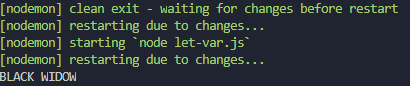
\includegraphics[width=10cm, height=2cm]{1.PNG}
\end{center}
A diferencia de \textbf{let} esta solo se puede asignar el nombre de una variable una única vez, si se vuelve a instanciar con el mismo esta dará error.
El uso de las variables let, es el que solo se instancia   dentro de la función donde se va usar y subfunciones que desciendan de estas, no pueden ser usadas por funciones superiores a estas.
\lstinputlisting[firstline=1,lastline=7,style=htmlcssjs]{codigo/let-var.js}
El resultado que obtendremos sera el siguiente:
\begin{center}
  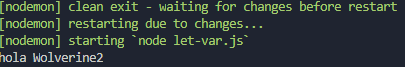
\includegraphics[width=10cm, height=1.5cm]{2.PNG}
\end{center}
Esto significa que la variable nombre no puede ser remplazada por la variable nombre instanciada dentro del  \textbf{if} por los que solo se imprime el nombre ya antes asignado.
\\
Las variables \textbf{let} si pueden ser usadas por funciones si estas son declaradas fuera de estas y así mismo pueden cambiar de valor si estas no han sido instanciadas dentro de la función.
\lstinputlisting[firstline=9,lastline=13,style=htmlcssjs]{codigo/let-var.js}
\begin{center}
  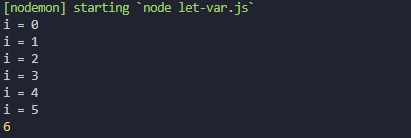
\includegraphics[width=10cm, height=3.5cm]{3.PNG}
\end{center}



\chapter{Templates}
El significado de templates dentro de lo que estamos estudiando, se refiere a como manipulamos los datos tipos cadenas.\\
En el siguiente ejemplo tenemos dos formas diferentes en la cual podemos crear variables con información ya antes obtenida.
\lstinputlisting[firstline=1,lastline=4,style=htmlcssjs]{codigo/templates.js}
En la primer podemos usar el signo \textbf{+} para concatenar las variables \textbf{nombre} y \textbf{real}.\\
En el segundo utilizamos los signos  \textbf{\$\{ variable \}} los cuales hacen referencia a la variable que se va a usar, esto evita mucho el uso de \textbf{""} poniendo dentro de uno solo.

Podemos tambien compara valores para saber si los contenidos de las dos varibales son iguales en estructura y contenido, y para esto usamos el \textbf{=== (tripe igual)}.
\lstinputlisting[firstline=1,lastline=6,style=htmlcssjs]{codigo/templates.js}
Obteniendo el resultado siguiente:
\begin{center}
  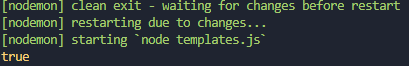
\includegraphics[width=10cm, height=1.5cm]{4.PNG}
\end{center}
El valor obtenido en la consola es un valor logico, diciendonos que el contenido y estructura son iguales.\\
Asi mismo podemos usar funciones utilizando estas variables
\lstinputlisting[firstline=1,lastline=10,style=htmlcssjs]{codigo/templates.js}
\begin{center}
  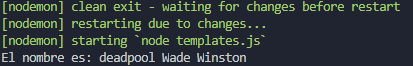
\includegraphics[width=10cm, height=1.5cm]{5.PNG}
\end{center}



\chapter{Destructuración}

Nos referimos a \textbf{destructuracion} al uso de variables como objetos, es decir usar variables para guardar diferentes tipos de variables, incluso usando atributos de esta variable como el siguiente ejemplo.
\lstinputlisting[firstline=1,lastline=9,style=htmlcssjs]{codigo/destructuracion.js}
En este ejemplo creamos la variable \textbf{deadpool} como una variable de destructuracion, dándole atributos como  \textbf{nombre, apellido, poder, e incluso asignándole una función} la cual retorna una cadena con todos los atributos antes mostrados con solo llamar a la variable y su función.
\begin{center}
  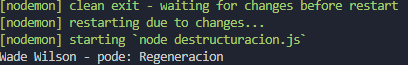
\includegraphics[width=10cm, height=1.5cm]{6.PNG}
\end{center}
Asi mismo podemos crear nuevas variables y asignarles los valores de los atributos ya insertados.
\lstinputlisting[firstline=1,lastline=11,style=htmlcssjs]{codigo/destructuracion.js}
\begin{center}
  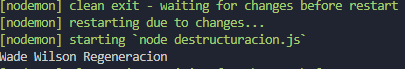
\includegraphics[width=10cm, height=1.5cm]{7.PNG}
\end{center}

\chapter{Flechas}

El uso de \textbf{flechas} ayuda mucho dentro del tema \textbf{optimización de código} lo cual es fundamental para el tema de uso de recursos.\\
Las flechas son prácticamente funciones optimizadas en código, así mismo a través de estas podemos enviar atributos, retornar valores y hacer operaciones.
\lstinputlisting[firstline=7,lastline=10,style=htmlcssjs]{codigo/flecha.js}
\begin{center}
  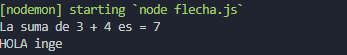
\includegraphics[width=10cm, height=1.5cm]{8.PNG}
\end{center}
Las \textbf{flechas}, así mismo se puede usar como una función normal dentro de una variable con atributos dentro.
\lstinputlisting[firstline=12,lastline=20,style=htmlcssjs]{codigo/flecha.js}
\begin{center}
  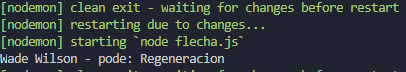
\includegraphics[width=10cm, height=1.5cm]{9.PNG}
\end{center}

\chapter{Funciones Callbacks} 
Una \textbf{función de callback} es una función que se pasa a otra función como un argumento, que luego se invoca dentro de la función externa para completar algún tipo de rutina o acción.
La funcionalidad principal del ejemplo a presentar, es el de presentar buscar a una persona mediante su id, mostrar su sueldo y en caso de no encontrarla mostrar un mensajes sobre la falla o error encontrado.\\
\begin{enumerate}
  \item Instanciaremos dos Variables tipo Array, la primara almacenara el id y nombre de los participantes, la segunda, el id y el sueldo que este recibe.
  \lstinputlisting[firstline=1,lastline=10,style=htmlcssjs]{codigo/callbacks2.js}
  \item Creación del callback getempleado
  \lstinputlisting[firstline=12,lastline=19,style=htmlcssjs]{codigo/callbacks2.js}
  \begin{enumerate}
    \item La variable getEmpleado almacena una función tipo flecha, recibiendo los atributos del id, y la función llamada callback,
    \item La variable empleadoDb recorre la variable empleados (ids y nombres) buscando cual id es igual al ingresado
    \item En la condición if, si la variable empeladoDb no tiene información (es decir no se encontró al empleado), ingresara dentro de la función callback el mensaje de \textbf{No existe empleado}
    \item Caso contrario retornara un valor nulo y la variable empleadoDB.
  \end{enumerate}
   \item Creacion callback getSalario
   \lstinputlisting[firstline=22,lastline=29,style=htmlcssjs]{codigo/callbacks2.js}
   \begin{enumerate}
    \item La variable getSalario guarda una función tipo flecha con los atributos a recibir de un objeto y una función desarrollarse.
     \item La variable salarioDB recorre el array salario (id y salario) antes creado hasta encontrar cual es igual al id del salario con el del empleado.
     \item En la sentencia if, si la variable no almaceno ningún valor (es decir que no se encontró) retornara un mensaje de error confirmando que no se encontró salario para tal usuario.
     \item En caso de si almacenar un valor, se ejecuta la función callback enviando como un objeto creado con el nombre del empleado y el salario que este recibe.
     \end{enumerate}
     \item Invocando a las funciones.
     \lstinputlisting[firstline=32,lastline=42,style=htmlcssjs]{codigo/callbacks2.js}
     \begin{enumerate}
        \item Invocamos la función getEmpleado enviando como parámetro un \textbf{id = 2} y el siguiente atributo que enviamos es una función recibiendo los atributos de \textbf{erro} y el de \textbf{empleadoDB}
         \item En la condición if, en caso de recibir un error, mandara a imprimir en consola
         \item caso de no recibir un error, invocara a la función getSalario, la cual envía al objeto \textbf{usuario} recibido(\textbf{empleadoDB}), y otra función dos atributos, uno de error y el con la respuesta.
         \item En caso de encontrar un error se nos imprimirá este, caso contrario obtendremos nuestra respuesta.
     \end{enumerate}
\end{enumerate}
\begin{center}
  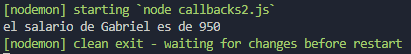
\includegraphics[width=10cm, height=1.5cm]{10.PNG}
\end{center}


\chapter{Promesas}
Una promesa es un objeto devuelto al cuál se adjuntan funciones callback, en lugar de pasar callbacks a una función.\\
El ejemplo a mostrar es el mismo que el anterior, realizado en callbacks pero ahora, se desarrollara con promesas.
\begin{enumerate}
  \item Inicializamos las variables empleados y salarios
  \lstinputlisting[firstline=1,lastline=9,style=htmlcssjs]{codigo/callbacks2.js}
  \item Promesa getEmpleado
  \lstinputlisting[firstline=10,lastline=19,style=htmlcssjs]{codigo/callbacks2.js}
  \begin{enumerate}
    \item Creamos la variable getEmpleado el cual almacena una función tipo flecha con instanciando dentro de su ejecución una promesa.
    \item Dentro de la promesa tenemos dos atributos a recibir \textbf{ resolve } (Si la función se cumple correctamente), \textbf{reject}(si ocurre algún error)
    \item Así mismo en la varible empleadoDB guardamos la búsqueda dentro del array empleados que tenga igual al id ingresado.
    \item En caso de no guardar ninguna información utilizaremos el atributo \textbf{reject} de la promesa para enviar un error
    \item Caso contrario utilizaremos el atributo \textbf{resolve} para enviar la respuesta.
  \end{enumerate}
  \item Promesa getSalario
  \lstinputlisting[firstline=21,lastline=31,style=htmlcssjs]{codigo/callbacks2.js}
  \begin{enumerate}
    \item Creamos la variable getSalario almacenando una función recibiendo los atributos empleado(objeto).
    \item Instanciamos una promesa con sus atributos \textbf{resolve} y \textbf{reject}
    \item la variable almacena el salario que pertenezca al empleado recibido a través de su id.
    \item en caso no almacenar ningún dato salarioDB se ejecuta el atributo \textbf{reject} enviando un mensaje de error
    \item Caso contrario Se crea un objeto guardando el nombre y sueldo del empleado.
  \end{enumerate}
  \item Invocacion de la promesa
  \lstinputlisting[firstline=44,lastline=48,style=htmlcssjs]{codigo/callbacks2.js}
  \begin{enumerate}
    \item Al invocar getEmpleado mandamos un id en este caso no valido.
    \item \textbf{.then} nos ayuda a identificar si la promesa se ejecutó con éxito, guardando el resultado en una variable llamada empleados.
    \item al ejecutarse con éxito la promesa getSalario es invocada mandamos la respuesta almacenada llamada empleados.
    \item \textbf{.catch()} nos ayuda atrapar los errores lanzados por las promesas almacenándolos en una variable llamada err.
  \end{enumerate}
\end{enumerate}
\begin{center}
  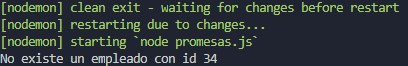
\includegraphics[width=10cm, height=1.5cm]{11.PNG}
\end{center}

\chapter{Async - Await}
Las funciones asíncronas utilizan la sintaxis async y await para esperar que una promesa sea resuelta.
En este capittulo usaremos el ejemplo del desarrollado en las promesas, pero implementando las sintaxis de \textbf{async-await}
\begin{enumerate}
  \item Inicializar variables empleados y salarios
  \lstinputlisting[firstline=1,lastline=9,style=htmlcssjs]{codigo/async-await.js}
  \item Inicializar promesa getEmpleado
  \lstinputlisting[firstline=11,lastline=18,style=htmlcssjs]{codigo/async-await.js}
  \begin{enumerate}
    \item A diferencia de las promesas al inicializar la función antes de los atributos agregamos la palabra async, la cual hacer referencia a que la función va a devolver una respuesta y va hacer capturada por un await en algún momento.
    \item pedimos de parámetros el id del empleado
    \item buscamos a que empleado le corresponde el id y guardamos en la variable empleadoDB.
    \item en caso de que no se encuentra creamos y lanzamos un error con el comando \textbf{throw}.
    \item en caso de si encontrarlo retornamos la respuesta que es un objeto.
  \end{enumerate}
  \item Inicializar promesa getSalario
  \lstinputlisting[firstline=20,lastline=27,style=htmlcssjs]{codigo/async-await.js}
  \begin{enumerate}
    \item Recibimos de atributo un objeto llamado empleado.
    \item Buscamos el salario que corresponda a tal empleado a través de sus ids.
    \item En caso no encontrar lanzamos un error con el comando \textbf{throw}
    \item Caso contrario se retorna un objeto con el nombre y salario del empleado.
  \end{enumerate}
  \item Inicializar  async getInformacion
  \lstinputlisting[firstline=32,lastline=36,style=htmlcssjs]{codigo/async-await.js}
  \begin{enumerate}
    \item Recibimos un atributo llamado id.
     \item creamos una variable llamado empleado, la cual con el comando await recibe la solución realizada por la promesa getEmpleado.
     \item Al crear una variable salario, junto con el comando await recibe la solución de la promesa a la cual se envía la variable empleado.
     \item Al final de la operación retornamos un mensaje con la solución 
  \end{enumerate}
  \item LLamada al async getInformacion
  \lstinputlisting[firstline=37,lastline=39,style=htmlcssjs]{codigo/async-await.js}
  \begin{enumerate}
    \item Llamamos al async getInformacion y el enviamos el id 1
    \item \textbf{.then()} nos ayuda a crear una variable (\textbf{mensaje}) la cual va a recibir la respuesta.
    \item \textbf{.catch()}nos ayuda a recibir los errores que son lanzados en el transcurso del código, imprimiendo en consola cual fue el error.
  \end{enumerate}
  
\end{enumerate}
\begin{center}
  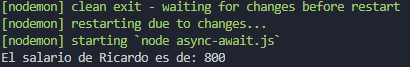
\includegraphics[width=10cm, height=1.5cm]{12.PNG}
\end{center}
\end{document} 